\documentclass[11pt,letterpaper, twocolumn]{article}
\setlength{\marginparwidth}{2cm}
\usepackage[english]{babel}
\usepackage[utf8x]{inputenc}
\usepackage{amsmath}
\usepackage{amssymb}
\usepackage{graphicx}
\usepackage{tikz}
\usepackage{esvect}
\usepackage[colorinlistoftodos]{todonotes}
\usepackage{enumitem}

\raggedbottom

\author{Etash Jhanji\\\small Collaborators: Josh (TA), Colin (TA), \\\small Nathan Banks, Rohan Dalal, Logan Balmer, Akpandu Ekezie}
\title{Physics HW 2}

\begin{document}
\maketitle

\section{The Invariant}
\begin{center}
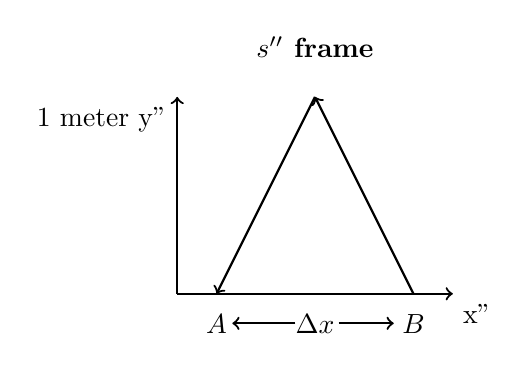
\begin{tikzpicture}
    \draw[thick,->] (0,0) -- (3.5,0) node[anchor=north west] {x''};
    \draw[thick,->] (0,0) -- (0, 2.5) node[anchor=north east] {1 meter y''};
    \node [label={[xshift=1.75cm, yshift=-0.75cm]$\Delta x$}]{};
    \node [label={[xshift=0.5cm, yshift=-0.75cm]$A$}]{};
    \node [label={[xshift=3cm, yshift=-0.75cm]$B$}]{};
    \draw[thick,->] (3,0) -- (1.75, 2.5) node[anchor=north west] {};
    \draw[thick,->] (1.75, 2.5) -- (0.5, 0) node[anchor=north east] {};
    \node [label={[xshift=1.75cm, yshift=2.75cm]\textbf{$s''$ frame}}]{};
    \draw[thick,->] (2.05, -0.75/2) -- (2.75, -0.75/2) node[anchor=north east] {};
    \draw[thick,->] (1.5, -0.75/2) -- (0.7, -0.75/2) node[anchor=north east] {};
\end{tikzpicture}
\end{center}
\begin{align*}
    &\Delta t^2 - (-\Delta x)^2\\
    &= (2\sqrt{1+\frac{\Delta x^2}{4}})^2 - (-\Delta x)^2\\
    &= (4-\Delta x)^2 - (\Delta x)^2\\
    &=4\\
\end{align*}
\begin{center}
\begin{tikzpicture}
    \draw[thick, ->] (-2, 0) -- (2,0) node[anchor=north west] {x};
    \draw[thick, ->] (0, 0) -- (0,3) node[anchor=north east] {t};
    \filldraw[black] (0,2) circle (2pt) node[anchor=north east]{B};
    \filldraw[black] (-1.5,2.5) circle (2pt) node[anchor=north east]{B''};
    \filldraw[black] (1.5,2.5) circle (2pt) node[anchor=north east]{B'};
\end{tikzpicture}
\end{center}

\section{Michelson-Morley experiment}
In the stationary frame speed, time, and length are constant
\begin{align*}
    L_x &= L_y\\
\end{align*}
In the frame with motion, though
\begin{align*}
    t_y &= 2\sqrt{l^2 + \frac{\Delta x^2}{4}}\\
    t_y &= 2\sqrt{l^2 + \frac{(\beta t_y)^2}{4}}\\
    t_y^2 &= 4({l^2 + \frac{(\beta t_y)^2}{4}})\\
    t_y^2 &= 4l^2 + \beta^2 t_y^2\\
    t_y^2 - \beta^2 t_y^2 &= 4l^2\\
    t_y^2 (1 - \beta^2)&= 4l^2\\
    t_y &= \frac{2l}{\sqrt{1-\beta^2}}\\
\end{align*}
\begin{align*}
    t_x &= \frac{l'}{1+\beta} + \frac{l'}{1-\beta} \\
    t_x &= \frac{l'[(1-\beta)+(1+\beta)]}{1-\beta^2}\\
    t_x &= \frac{2l'}{1-\beta^2}\\
\end{align*}
\begin{align*}
    l &= \gamma l'\\
    l' &= \frac{l}{\gamma}\\
    t_x &= \frac{2l}{\gamma(1-\beta^2)}\\
    t_x &= \frac{2l\sqrt{1-\beta^2}}{1-\beta^2}\\
    t_x &= \frac{2l}{\sqrt{1-\beta^2}}\\
    t_x &= t_y\\
\end{align*}


\section{Moving Balls}
\begin{center}\textbf{B} because the length contraction will occur on the axis of movement. \end{center}

\section{Provisions in space}
\begin{align*}
    \beta &= \frac{1}{2}\\
    \gamma &= \frac{1}{\sqrt{1-0.5^2}}\\
    \gamma &= \frac{1}{\sqrt{0.75}}\\
    t&=20\text{ years}\\
    20 &= \gamma t\\
    t &= 20 \sqrt{0.75}\\
    t &= 10 \sqrt{3} \text{ years}\\
    t &= 6322 \text{ days}\\
\end{align*}
\begin{center}6322 meals. \end{center}

\section{Velocity Addition}
\begin{align*}
    \beta_x &= \frac{\beta_x' + \beta}{1+\beta\beta'}\\
    \beta_x' &=\frac{\beta_x'' + \beta'}{1+\beta'\beta_x''}\\
    \beta_x' &=\frac{0.9 + 0.9}{1+0.9(0.9)}\\
    \beta_x' &=0.994475\\
    \beta_x &= \frac{(0.994475) + 0.9}{1+0.9(0.994475)}\\
    \beta_x &= 0.999708c
\end{align*}


\section{Break down of Galilean Transformations}
\begin{align*}
    t' &= \gamma t\\
    0.99t &= t\sqrt{1-\beta^2}\\
    0.99 &= \sqrt{1-\beta^2}\\
    0.99^2 &= 1-\beta^2\\
    \beta &= \sqrt{1-0.99^2}\\
    \beta &= 0.141\\
\end{align*}
\begin{center}$0.141c$\end{center}

\section{Temporal order}
All time-like events are in theory physically possible. In this case all time like events can be mapped to each other by Lorentz transformations and preserve the order where an event A that causes B will occur before B. Similarly light-like scenarios, with sufficient distance, will be able to preserve order of events. The issue comes when you reach space-like intervals where you exceed the speed of light. This is obviously impossible to physically happen, but also breaks down causation because if A is to occur, it will have caused B before it happens. 

\section{Euclidean “slope” transformations}
\begin{align*}
    \begin{pmatrix}x\\y\end{pmatrix} &= \begin{pmatrix}G&-BG\\BG&G\end{pmatrix}\begin{pmatrix}x'\\y'\end{pmatrix}\\
    \begin{pmatrix}x\\y\end{pmatrix}&=\begin{pmatrix}Gx' - BGy' \\ BGx'+Gy'\end{pmatrix}\\
    x&=Gx' - BGy'\\
    x&=Gx' - Gy'\tan\theta\\
    G & \equiv \frac{1}{\sqrt{1+B^2}}\\
    G &= \frac{1}{\sqrt{1+\tan^2\theta}}\\
    G &= \cos\theta\\
    x&=x'\cos\theta - y'\cos\theta\tan\theta\\
    x&=x'\cos\theta - y'\sin\theta\\
    y&=x'\sin\theta+y'\cos\theta\\
\end{align*}
\begin{align*}
    &\sqrt{x^2+y^2}\\
    &=\sqrt{(x'\cos\theta - y'\sin\theta)^2+(x'\sin\theta+y'\cos\theta)^2}\\
    % &=\sqrt{x'^2\cos^2\theta + y'^2\sin^2\theta - 2x'y'\cos\theta\sin\theta +x'^2\sin^2\theta+y'^2\cos^2\theta + 2x'y'\cos\theta\sin\theta}\\
    &=\sqrt{x'^2\cos^2\theta + y'^2\sin^2\theta +x'^2\sin^2\theta+y'^2\cos^2\theta}\\
    &=\sqrt{x'^2(\cos^2\theta + \sin^2\theta) + y'^2(\sin^2\theta +\cos^2\theta)}\\
    &=\sqrt{x'^2+ y'^2}\\
\end{align*}

\end{document}